\documentclass[a4paper,10pt]{article}
% UTF8 Charset für Umlaute/Sonderzeichen
\usepackage[utf8]{inputenc}
% Deutsche Namen und Datumsformat
\usepackage[ngerman]{babel}
%Quellenangaben
\usepackage{hyperref}
%Fancy Mathesymbole
\usepackage{amssymb}
\usepackage{dsfont}
%Aufzählung
\usepackage{paralist}
%Pfeile
\usepackage{amsmath}
\makeatletter
\newcommand{\xRightarrow}[2][]{\ext@arrow 0359\Rightarrowfill@{#1}{#2}}
\makeatother
%Krams
\usepackage{amsmath}
\usepackage{amsthm}
%Gewitter
\usepackage{ stmaryrd }
% Algorithmen Pseudocode
\usepackage[]{algorithm2e}
% Bilder
\usepackage{graphics}
\usepackage{wrapfig}
%GeoGebra
\usepackage{tikz}
\usepackage{tkz-euclide}
\usetikzlibrary{arrows,automata,positioning}

\tikzset{
	state/.style={
		circle,
		draw=black, very thick,
		minimum height=2em,
		inner sep=2pt,
		text centered,
	},
}



\newcommand{\bigo}{\ensuremath{\mathcal{O}}}
\newcommand{\BT}{\ensuremath{\Theta}}
\newcommand{\N}{\ensuremath{\mathbb{N}}}
\newcommand{\Set}{\ensuremath{\mathcal{S}}}
\newcommand{\PMenge}{\ensuremath{\mathcal{P}}}
\newcommand{\xp}{\ensuremath{x_{pre}}}
\newcommand{\yp}{\ensuremath{y_{pre}}}


% Hier die Nummer des Blatts, Autoren und Name des Betreuers angeben.
\newcommand{\blatt}{10}
\newcommand{\autor}{Edenfeld, Lemke, Moser, Schinke}
\newcommand{\betreuer}{Carina Pilch}
\usepackage{../abgabe}

\begin{document}
	% Seitenkopf mit Informationen
	\kopf
	
	\aufgabe 1

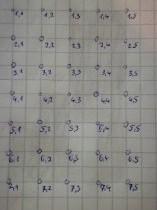
\includegraphics[width=0.33\textwidth]{1a.jpeg}


\subsection*{Aufgabenteil a:}
$v=\{(2,3),(2,4),(3,3),(3,4),(4,3),(4,4),(5,2),(5,3),(5,4),(6,1),(6,2),(6,4),(7,1),(7,2),(7,3),(7,4)\}$

\subsection*{Aufgabenteil b:}

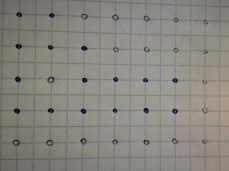
\includegraphics[width=0.33\textwidth, angle=90]{1b.jpeg}
	
	\aufgabe 2

\begin{align*}
\{l_2, l_3, l_5\} &\vDash p \vee q \\
\emptyset &\vDash AG(p \vee q) \\
\emptyset &\vDash EFAG(p \vee q)
\end{align*}

Da keine Location $AG(p\vee q)$ erfüllt, erfüllt auch keine $EFAG(p\vee q)$.
	
	\aufgabe 3

\begin{enumerate}
\item Die Lineare Transformation wird genutzt, um das nächste Segment der flowpipe zu berechnen.
\item Der Membershiptest wird genutzt, um die Einhaltung der geltenden Invarianten zu überprüfen.
\item Die Durchschnittsbildung und die Minkowski Summe werden für die Durchführung diskrete Sprünge verwendet. Die Durchschnittsbildung garantiert dabei die Einhaltung der relevanten Guards.
\item Das initiale Segment wird durch Bildung einer konvexen Hülle um die Vereinigung von X0 und der Menge der im ersten Zeitsegment erreichbaren Punkten gebildet.
\item Test for emptiness
\end{enumerate}

	
	\aufgabe 4

Stopwatch Automaton:

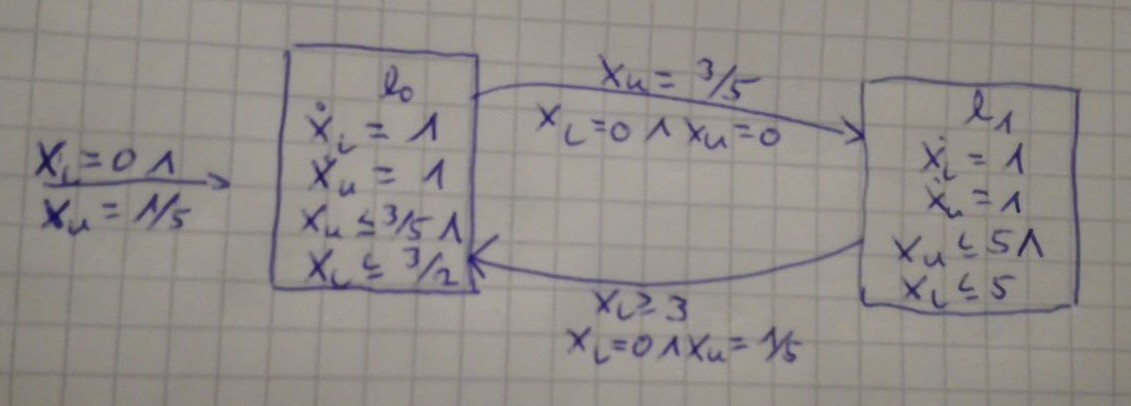
\includegraphics[width=\textwidth]{4.jpeg}

Stopwatch automaton is already timed automaton.
	
	\aufgabe 5

\begin{align*}
T_{l_0}^+(\varphi) = &\exists\xp.\exists\yp.\exists t. t\ge 0\wedge\xp=0\wedge\yp=0\wedge \xp +2t\leq x\leq \xp +4t\wedge\\&\yp +t\leq y\leq\yp + 2t\wedge x\leq 20\wedge y\leq 20\\
=&\exists t. t\ge 0\wedge 2t\leq x\leq 4t\wedge t\leq y\leq 2t\wedge x\leq 20\wedge y\leq 20\\
=&0\leq x\wedge 0\leq y\wedge y\leq x\wedge \frac{x}{4}\leq y\wedge x\leq 20\wedge y\leq 20\\
=&0\leq x\leq 20\wedge 0\leq y\leq 20\wedge y\leq x\wedge \frac{x}{4}\leq y\\\\
D_e^+(\varphi)=&\exists\xp.\exists\yp.0\leq \xp\leq 20\wedge 0\leq \yp\leq 20\wedge \yp\leq \xp\wedge \frac{\xp}{4}\leq \yp\wedge\xp=20\\&\wedge x=1\wedge y=1\wedge x\leq 20\wedge y\leq 20\\
=&\exists\yp.0\leq \yp\leq 20\wedge \yp\leq 20\wedge 5\leq \yp\wedge x=1\wedge y=1\\
=&\exists\yp.5\leq \yp\leq 20\wedge x=1\wedge y=1\\
=&x=1\wedge y=1\\\\
T_{l_0}^+(\varphi) = &\exists\xp.\exists\yp.\exists t. t\ge 0\wedge\xp=1\wedge\yp=1\wedge \xp +2t\leq x\leq \xp +4t\wedge\\&\yp +t\leq y\leq\yp + 2t\wedge x\leq 20\wedge y\leq 20\\
=&\exists t. t\ge 0\wedge 1+2t\leq x\leq 1+4t\wedge 1+t\leq y\leq 1+2t\wedge x\leq 20\wedge y\leq 20\\
=& 1\leq x\leq 20\wedge 1\leq y\leq 20 \wedge y\leq x \wedge \frac{x}{4}\leq y +\frac{3}{4}
\end{align*}

	 
\end{document}

